\documentclass[conference]{IEEEtran}
\IEEEoverridecommandlockouts

\usepackage{cite}
\usepackage{amsmath,amssymb}
\usepackage{booktabs}
\usepackage{graphicx}
\usepackage{xcolor}
\usepackage{url}
\usepackage[hidelinks]{hyperref}
\usepackage{tikz}
\usetikzlibrary{arrows.meta, positioning}

\newcommand{\code}[1]{\texttt{#1}}

\begin{document}

\title{Measuring LLM Security Verdicts: Coverage, Abstention,\\ and Adversarial Suppression}

\author{%
\IEEEauthorblockN{S.V.Divya}
\IEEEauthorblockA{Department of CSE,\\
K.P.R College of Engineering\\
and Technology,\\
Coimbatore-642109.\\
divyasvvsb@gmail.com}
\and
\IEEEauthorblockN{R Harshan}
\IEEEauthorblockA{Department of CSE,\\
K.P.R College of Engineering\\
and Technology,\\
Coimbatore-642109.\\
harshanr695@gmail.com}
\and
\IEEEauthorblockN{P.M Akhil Jeikar}
\IEEEauthorblockA{Department of CSE,\\
K.P.R College of Engineering\\
and Technology,\\
Coimbatore-642109.\\
akhiljeikar06@gmail.com}
\and
\IEEEauthorblockN{T Ezhilperungo}
\IEEEauthorblockA{Department of CSE,\\
K.P.R College of Engineering\\
and Technology,\\
Coimbatore-642109.\\
ezhilperungotamizhazhagan@gmail.com}
\and
\IEEEauthorblockN{M Gurunathan}
\IEEEauthorblockA{Department of CSE,\\
K.P.R College of Engineering\\
and Technology,\\
Coimbatore-642109.\\
gurunathanmofficial@gmail.com}
}

\maketitle

\begin{abstract}
Large language models (LLMs) are increasingly used as \emph{verifiers} of security
findings: a static analyzer proposes a candidate and a model adjudicates whether it
is real. Whether such a verdict can be trusted is rarely measured. We adapt the
\emph{four-way decomposition}---an instrument previously used to show that static
analyzers flag constructs rather than vulnerabilities---to LLM verifiers and extend
it with evidence gating, an adversarial comment attack, a composition study, and a
calibration analysis. On a 151-pair real-fix security stratum from JavaVFC, an
evidence-grounded verifier tracks the fix on 17.6\% of pairs (95\% CI [16.7,18.5],
$k{=}5$) against 0.7\% for the pattern matcher it is meant to replace and 0\% for
CodeQL, with exact McNemar $p{<}10^{-7}$ against both---yet it abstains on 51.5\%
of judgements and misses 79.1\% of genuine fixes, so its bottleneck is
\emph{coverage}, not accuracy. Gating costs no recall (3:4, $p{=}1.0$) and removes
ungrounded positives; a blinded-message ablation shows the commit message leaks
$-18.1$ points of detection, an LLM still detects ${\sim}19\times$ the tool on
code alone. Adversarial comments evade 12--20\%, every successful evasion is an
\emph{abstention} rather than a false positive, and stripping comments does not
help: an attacker need only make the verifier unsure, not wrong. Calibration at
scale is mediocre (ECE 0.116) and accuracy on a labelled benchmark does not
improve over the analyzer. Our scaled evidence spans one model family on the
stratum plus a cross-family replication on the legacy subset, and we state the
remaining limits plainly. We release a reproducible harness and argue that
abstention and coverage should be reported as first-class outcomes of security
agents.
\end{abstract}

\begin{IEEEkeywords}
abstention, adversarial robustness, calibration, syntax graphs,
evidence grounding, large language models, program analysis, selective
prediction, static analysis, vulnerability verification.
\end{IEEEkeywords}

\section{Introduction}
Automated vulnerability analysis has converged on a standard shape: a policy
queries tools and a code graph and is trained or prompted to report findings
\cite{vulagentrl,antares,eava,openant}. LLM agents now drive that loop---reasoning
over repositories, invoking analyzers, and drafting fixes. In each case a model
makes \emph{verification} judgements: given a candidate produced by a scanner, a
fuzzer, or another model, is it real? As agents take over the gate between a
warning and a fix, the question becomes whether their verdicts can be trusted.

That question is harder than it looks. A model can be right about the code and
wrong about the vulnerability: it can flag a dangerous-looking construct that the
patch did not touch, agree that a benchmark sample is vulnerable without reasoning
about the vulnerability, or become confident on inputs unlike its training
distribution. For a static analyzer, \emph{our companion study} showed
that the fraction of commits whose verdict \emph{moves with a fix} can be two
orders of magnitude below its benchmark true-positive rate, and introduced the
\emph{four-way decomposition} to make that gap visible \cite{sastaudit}. We ask the
same of LLM verifiers.

The stakes are concrete. Static analysis has always lived with false positives
\cite{sadowski2018lessons}, and machine-learning vulnerability detectors inherit the
same label and validity problems \cite{chakraborty2022deep,croft2023data,
arp2022dos}. When a model is placed in front of remediation, two failures are
possible: it can \emph{confirm} a non-vulnerability (wasted effort, eroded trust)
or, more dangerously, \emph{suppress} a real one. Prior work shows that LLM
security detectors are easily steered by adversarial comments \cite{alibi} and by
indirect prompt injection \cite{greshake2023not}; what has not been measured
systematically is whether an LLM \emph{verdict} tracks the vulnerability at all, how
it fails when it does not, and how it behaves under composition and an adversary.

\noindent\textbf{Contributions.}
\begin{itemize}
\item \textbf{An instrument.} We give the first systematic application of the
four-way decomposition --- introduced in our companion study for static
analyzers \cite{sastaudit} --- to LLM verifiers, gate every verdict on
machine-checkable evidence, split adversarial evasion by outcome
(false positive vs.\ abstention), and report the coverage of the process.
The harness, corpora, and pinned analyzers are released.
\item \textbf{A coverage-bound finding.} An evidence-grounded verifier tracks the
fix 17.6\% of the time (95\% CI [16.7,18.5], $k{=}5$) against 0.7\% for the pattern
matcher (which over-reports $10\times$) and 0\% for CodeQL---exact McNemar
$p{<}10^{-7}$ against both---yet it abstains on 51.5\% of judgements and misses
79.1\% of genuine fixes. Its bottleneck is \emph{silence}, not error---a profile
that precision-only evaluation cannot see.
\item \textbf{Abstention as the attack surface.} Under adversarial comments, every
successful evasion is an abstention rather than a false positive; stripping
comments as a mitigation does not reduce evasion. An attacker need only make the
verifier unsure, not wrong.
\item \textbf{Leakage is measurable.} Blanking the commit message drops detection
on the same pairs from 31.4\% to 13.3\% ($-18.1$ points): the message is a real
label channel, and code alone still detects ${\sim}19\times$ the tool.
\item \textbf{Composition relocates trust.} Evidence gating costs no recall
(3:4, $p{=}1.0$) and marginally removes ungrounded positives; requiring agreement
with a weaker deterministic verifier loses recall and gains nothing.
\item \textbf{A negative result on labelled ground truth.} On OWASP Benchmark
(2{,}740 labelled cases) the analyzer reaches recall 0.905 / precision 0.734, but
the LLM verifier does not improve precision: in a matched sample neither a local
7B nor a cloud model rejects false positives (0--2 of 15), and blinding the
scanner hint only raises abstention. Verification is coverage-bound.
\item \textbf{Calibration and cost.} At $n{=}151$ the verifier is nearly precise
(0.9\% fixed-side false positives) but not reliably calibrated (ECE 0.116
[0.106, 0.131]); disabling model thinking cuts cost ${\sim}8\times$ at a measured
precision cost, and a content-addressed verdict cache removes 100\% of repeat
cost.
\end{itemize}

We are explicit about what the scaled evidence does and does not cover
(Section~\ref{sec:threats}) and treat the paper as a measurement-methodology
contribution rather than a claim of a large effect.

\section{Background and Related Work}
\subsection{LLM agents for vulnerability analysis}
A fast-moving line of systems couples LLMs with static analysis, symbolic
execution, and fuzzing. OpenAnt decomposes code and adversarially verifies
candidates \cite{openant}, and agentic pipelines such as VulAgentRL, Antares, and
EAVA ground discovery in analyzers and code graphs \cite{vulagentrl,antares,eava}.
These systems report improved discovery, but they generally do not measure whether
a \emph{verdict} tracks the vulnerability, and they rarely report the
coverage--precision trade-off of the verifier itself. We measure the verdict rather
than the discovery rate.

\subsection{Verifiers and verifiable rewards}
VulAgentRL uses a code property graph both as a tool and as a reward verifier with
exact node matching \cite{vulagentrl}; Antares trains small models with verifiable
rewards \cite{antares}; EAVA couples supervised tuning with reinforcement learning
and requires evidence for a verdict \cite{eava}. ``Verifiable'' here means that the
training signal can be checked, not that the model's inference-time verdict is
grounded. We do not train; we ask what trust a grounded verdict earns at inference
time and how it fails.

\subsection{Adversarial robustness of LLM code analysis}
ALIBI shows that adversarial source comments defeat LLM vulnerability detectors
with high success rates \cite{alibi}; indirect prompt injection compromises
tool-integrated agents \cite{greshake2023not}; and code security-hardening work
demonstrates both the risk and partial defenses \cite{he2023large}. Earlier work
established that AI code assistants frequently produce insecure code
\cite{pearce2022asleep,perry2023do}. We attack the \emph{verifier} rather than the
detector, split evasion by outcome (false positive vs.\ abstention), and include an
adaptive attacker.

\subsection{Abstention, selective prediction, and calibration}
Selective classification makes rejection an explicit learning problem
\cite{geifman2017selective}, and out-of-distribution detection is the closely
related recognition task \cite{hendrycks2017baseline}. Modern neural networks are
often miscalibrated \cite{guo2017calibration}, and abstention has become a
first-class topic for LLMs, where models can partially ``know what they know''
\cite{kadavath2022language}; recent surveys catalogue the design space
\cite{wen2025know}. We bring this lens to security verification and show that abstention is not merely a safety valve---it is
the dominant adversarial target and the verifier's main bottleneck.

\subsection{LLM-as-a-judge reliability}
Using a model to adjudicate another model's output is now standard
\cite{zheng2023judging,liu2023geval}, and its failure modes are documented:
evaluators are order- and format-sensitive \cite{wang2024fair} and favour their own
generations \cite{panickssery2024llm}. Security verification is a judge problem in
this sense, but the ground truth is a code change rather than a preference; we
exploit that difference by scoring verdicts against the fix.

\subsection{Static analysis false positives and measurement validity}
Static analysis has been deployed at scale \cite{sadowski2018lessons}, and its false
positives are a persistent obstacle in practice. Machine learning for security
inherits methodological pitfalls---leakage, temporal bias, and ill-defined
labels \cite{arp2022dos}---and vulnerability datasets in particular are noisy
\cite{croft2023data}. Classical and learned vulnerability detectors and their
limits are well studied \cite{zhou2019devign,chakraborty2022deep,
ding2025vulnerability}. The OWASP Benchmark is the standard scanner yardstick
\cite{owaspbench}; our companion study showed its score is not well defined and does
not predict real detection, and introduced the four-way decomposition
\cite{sastaudit}. We extend \cite{sastaudit} from static tools to LLM verifiers.

\subsection{Code property graphs and query engines}
Program-analysis tooling exposes relational views of code: code property graphs
\cite{yamaguchi2014modeling} and object-oriented query languages over relational
data \cite{avgustinov2016ql} are the basis of modern taint engines. Our evidence
gating uses a lightweight tree-sitter graph rather than a sound dataflow engine;
Section~\ref{sec:threats} treats the resulting weakness explicitly.

\subsection{Ensembles and composition}
Combining predictors is a classical idea \cite{breiman1996bagging}, and diversity is
the property that makes an ensemble work \cite{kuncheva2003measures}. Our
composition result is a negative instance of that principle in a security setting:
adding a \emph{weaker} verifier by consensus does not add diversity, it adds the
weaker verifier's blind spot.

\section{Method}
Figure~\ref{fig:arch} shows the pipeline end to end. A revision pair is scanned
by a pinned analyzer; each candidate becomes a bounded verdict request; the verifier
must ground its verdict in resolvable evidence; the vulnerable and fixed verdicts are
then decomposed and summarised. An adversary can inject comments before verification.

\begin{figure}[t]
\centering
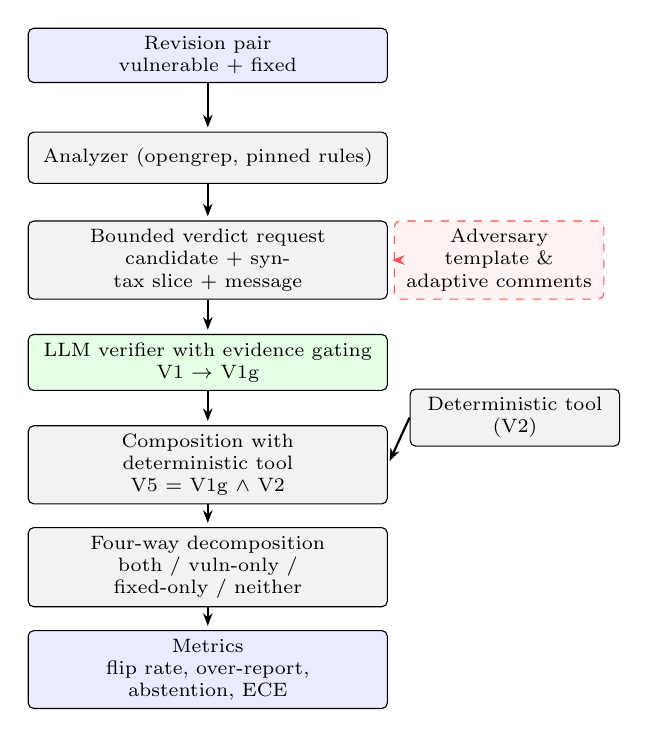
\begin{tikzpicture}[
  font=\scriptsize,
  >=Latex,
  box/.style={draw, rounded corners=2pt, align=center, inner sep=3pt,
              text width=4.35cm, minimum height=6.5mm},
  sidebox/.style={draw, rounded corners=2pt, align=center, inner sep=3pt,
                  text width=2.45cm, minimum height=6.5mm},
  io/.style={box, fill=blue!8},
  proc/.style={box, fill=black!5},
  ver/.style={box, fill=green!10},
  advbox/.style={sidebox, dashed, draw=red!70, fill=red!5},
  ar/.style={-{Stealth[length=1.6mm,width=1.2mm]}, thick, shorten >=1.5pt},
  dar/.style={-{Stealth[length=1.6mm,width=1.2mm]}, thick, dashed, red!70, shorten >=1.5pt}
]
\node[io]   (rev)   at (0,0)     {Revision pair\\ vulnerable $+$ fixed};
\node[proc] (an)    at (0,-1.3)  {Analyzer (opengrep, pinned rules)};
\node[proc] (req)   at (0,-2.6)  {Bounded verdict request\\ candidate $+$ syntax slice $+$ message};
\node[ver]  (judge) at (0,-3.9)  {LLM verifier with evidence gating\\ V1 $\rightarrow$ V1g};
\node[proc] (comp)  at (0,-5.2)  {Composition with deterministic tool\\ V5 $=$ V1g $\wedge$ V2};
\node[proc] (dec)   at (0,-6.5)  {Four-way decomposition\\ both / vuln-only / fixed-only / neither};
\node[io]   (met)   at (0,-7.8)  {Metrics\\ flip rate, over-report, abstention, ECE};

\node[advbox] (adv)  at (3.7,-2.6)  {Adversary\\ template \& adaptive comments};
\node[sidebox, fill=black!5] (tool) at (3.9,-4.6) {Deterministic tool\\ (V2)};

\draw[ar]  (rev)--(an);
\draw[ar]  (an)--(req);
\draw[ar]  (req)--(judge);
\draw[ar]  (judge)--(comp);
\draw[ar]  (comp)--(dec);
\draw[ar]  (dec)--(met);
\draw[dar] (adv.west)--(req.east);
\draw[ar]  (tool.west)--(comp.east);
\end{tikzpicture}
\caption{RewardAudit architecture. A revision pair is scanned by a pinned analyzer;
each candidate is turned into a bounded verdict request over a tree-sitter syntax
graph and the commit message. The verifier must ground its verdict in
resolvable evidence (V1$\rightarrow$V1g). An adversary (dashed) can inject comments
before verification, and a deterministic tool can be composed with the verifier.
Verdicts on the two revisions feed the four-way decomposition, which yields the
reported metrics.}
\label{fig:arch}
\end{figure}

\subsection{The four-way decomposition}
For a vulnerable/fixed revision pair, we classify a verifier's verdict into one of
four cells (Fig.~\ref{fig:cells}). Only \emph{vuln-only} is evidence of detection;
\emph{both} means the verifier flagged a construct present before \emph{and} after
the fix, so its verdict could not have been about the vulnerability. From the cells
we derive the \emph{flip rate} (vuln-only fraction), the \emph{naive coverage}
(fraction flagged on the vulnerable revision), and their ratio, the \emph{over-report
factor},
\begin{equation}
\text{over-report} = \frac{\text{naive coverage}}{\text{flip rate}}
                    = \frac{\text{both} + \text{vuln-only}}{\text{vuln-only}},
\end{equation}
so ``over-reports $6\times$'' means six findings on the vulnerable side for
every one that tracks the fix.

\begin{figure}[t]
\centering
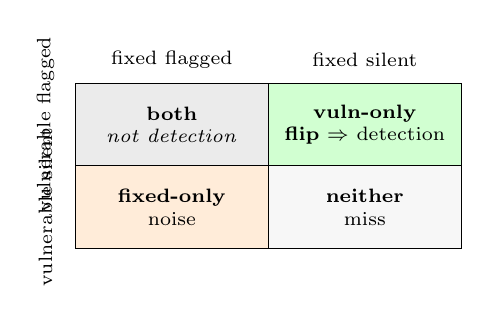
\begin{tikzpicture}[font=\scriptsize, x=1cm, y=1cm]
\def\w{2.45}\def\h{1.05}
% top row: vulnerable revision flagged
\draw[fill=black!8] (0,\h) rectangle (\w,2*\h);
\node[align=center] at (0.5*\w,1.5*\h) {\textbf{both}\\ \emph{not detection}};
\draw[fill=green!18] (\w,\h) rectangle (2*\w,2*\h);
\node[align=center] at (1.5*\w,1.5*\h) {\textbf{vuln-only}\\ \textbf{flip} $\Rightarrow$ detection};
% bottom row: vulnerable revision silent
\draw[fill=orange!15] (0,0) rectangle (\w,\h);
\node[align=center] at (0.5*\w,0.5*\h) {\textbf{fixed-only}\\ noise};
\draw[fill=black!3] (\w,0) rectangle (2*\w,\h);
\node[align=center] at (1.5*\w,0.5*\h) {\textbf{neither}\\ miss};
% headers
\node[align=center] at (0.5*\w, 2*\h+0.3) {fixed flagged};
\node[align=center] at (1.5*\w, 2*\h+0.3) {fixed silent};
\node[rotate=90, align=center] at (-0.38, 1.5*\h) {vulnerable flagged};
\node[rotate=90, align=center] at (-0.38, 0.5*\h) {vulnerable silent};
\end{tikzpicture}
\caption{The four-way decomposition over a revision pair. Only \emph{vuln-only} is
detection; \emph{both} means the verifier flagged a construct present before and
after the fix.}
\label{fig:cells}
\end{figure}

\subsection{Verifier arms}
We compare four arms on identical inputs.
\textbf{V1 (LLM, ungated)}: the model's verdict is taken as-is.
\textbf{V1g (LLM, gated)}: every cited evidence reference must resolve to a real
syntax node, or a positive verdict is downgraded to \emph{unknown}.
\textbf{V2 (tool)}: the pinned analyzer's verdict.
\textbf{V5 (hybrid)}: flagged only if the gated LLM \emph{and} the tool agree.

\subsection{Bounded verdict request and evidence gating}
The model never sees a repository. For a candidate it receives a bounded request:
the candidate (rule, location, CWE hint), the enclosing function extracted from a
tree-sitter syntax graph, and the commit message as legitimate context. It
must respond with a strict JSON verdict, cite \code{path:line} references, and may
answer \code{unknown\_risk}. Each reference is resolved against the graph; an
unverifiable positive is downgraded. Gating checks exactly one thing: that the
cited \code{path:line} exists and the enclosing function resolves. It does
\emph{not} verify taint flow, reachability, or any semantic property of the
data --- a lightweight syntax graph is not a dataflow engine, and we do not
pretend otherwise (Section~\ref{sec:threats}). We deliberately never feed
whole files by default, since that is the strawman this measurement is meant
to beat.

\subsection{Adversary}
\emph{Templates:} five plausible comment strategies (authority, sanitizer,
tool-output, test-passed, reviewed) inserted just above the suspected sink.
\emph{Adaptive:} an attacker model writes a comment, observes the verifier's
verdict, and refines over up to three rounds \cite{alibi}. We split evasion into
\emph{false-positive} and \emph{abstention} outcomes, because they target different
failure modes and demand different defenses.

\subsection{Calibration, selective risk, and cost}
Per revision judgement we record confidence, correctness, and disposition. We
compute expected calibration error (ECE), reliability bins, and a
selective-risk/coverage curve \cite{geifman2017selective}, plus false-negative rate
on vulnerable revisions and false-positive rate on fixed revisions. Cost is reported
in tokens and, at known prices, dollars per true positive.

\subsection{A worked example}
Consider an analyzer warning on \code{os.system(command)} in a helper reached from an
HTTP handler that reads an environment variable. An ungated model may answer
\emph{true positive} with a plausible but unfalsifiable rationale. Under V1g it must
cite a graph node for the source and the sink; if the cited nodes do not exist or
the call path is not present, the positive is downgraded to \code{unknown\_risk}.
This is the mechanism that produces the coverage--precision profile in
Section~\ref{sec:results}: grounding removes unverifiable positives, but a model
that cannot produce verifiable evidence abstains, and abstention is scored as a
miss on a fixed-side test.

\section{Experimental Setup}
\label{sec:setup}
\textbf{Corpora.} (i) JavaVFC \cite{javavfc} (784 commits; 327 usable
single-file; 324 materialised offline) screened to a \emph{security stratum of
151 revision pairs}: a security keyword in the commit \emph{subject} plus a
second out-of-band match (screen version recorded in the manifest), built as a
running-100 census plus a 51-pair extension. Every stratum result below uses
these 151 pairs unless noted. The hand-picked strong-security subset of 21 pairs
from our companion study \cite{sastaudit} is retained for cross-family
replication and for comparison with the original $k{=}5$ measurement. (ii) 5
hand-built Python vulnerable/fixed pairs and 3 canaries. (iii) The prior study's
21-file Java control set (18 vulnerable, 3 safe) \cite{sastaudit}. Each revision
is presented as an isolated file; the commit message is supplied as candidate
context, as a bug report would be, and is removed only in the blinded-message
ablation.

\textbf{Analyzers.} opengrep 1.30.0 with the prior study's pinned 690-rule Java
ruleset (sha256 \code{77df32e0\dots}) and a minimal 5-rule Python ruleset.
CodeQL 2.27.0 with the \code{java-security-extended} suite runs per pair (both
revisions in an isolated no-build database); a whole-directory database is
inapplicable on this corpus---the javac extractor is OOM-killed at ${\sim}300$
files---and we validated the per-pair adapter by reproducing the prior study's
finding on a known pair.

\textbf{Models.} Five families via an OpenAI-compatible API: \code{gpt-oss-120b},
\code{gpt-oss-20b}, \code{qwen3.8-27b}, \code{deepseek-flash},
\code{deepseek-v4-pro}. The 151-pair stratum runs use \code{mimo-v2.6-flash}
($k{=}5$, verdict cache disabled); the legacy 21-pair subset is run with both
\code{mimo-v2.6-flash} and \code{deepseek-flash} ($k{=}5$ each) for the
cross-family replication; the remaining families are checked on the 5-pair
Python set.

\textbf{Metrics and statistics.} For each arm we report the mean over $k{=}5$
independent runs with 95\% bootstrap intervals; because reasoning models are
non-deterministic even at temperature 0, we report the observed range alongside
the interval. Per-pair majority verdicts are compared with the exact McNemar
test on the same 151 pairs. Over-report is
$(\text{both}+\text{vuln\_only})/\text{vuln\_only}$.

\textbf{Reproducibility.} All assets are pinned by hash (\code{pins.json}); the
control reproduction and the Python-pair measurement run fully offline; 158 unit and
integration tests accompany the harness.

\section{Results}
\label{sec:results}
\subsection{Verifier dependence}
On identical inputs, models disagree in both flip rate and failure mode; the
cross-language check is summarised in Table~\ref{tab:cross}. \code{gpt-oss-120b}
flipped on 4/5 pairs and flagged a safe canary; \code{gpt-oss-20b} and \code{qwen}
and \code{deepseek-flash} flipped on 5/5 with one family showing a canary false
positive; \code{deepseek-v4-pro} abstained on one vulnerable revision. The result is
verifier-dependent---the phenomenon the instrument is designed to expose. The same
holds at scale: within one configuration repeated five times on the stratum, the
flip rate's 95\% interval is [16.7, 18.5]\% while the legacy 21-pair subset spans
28.6--38.1\% across runs (Section~\ref{sec:threats}), so even one model does not
have a stable point value.

\begin{table}[t]
\centering
\caption{Cross-family verdicts on 5 Python pairs / 3 canaries.}
\label{tab:cross}
\small
\begin{tabular}{@{}lccc@{}}
\toprule
Model & flip rate & both & canary FP \\
\midrule
gpt-oss-120b & 80\% & 1 & 1/3 \\
gpt-oss-20b & 100\% & 0 & 1/3 \\
qwen3.8-27b & 100\% & 0 & 0/3 \\
deepseek-flash & 100\% & 0 & 0/3 \\
deepseek-v4-pro & 80\% & 0 & 0/3 (1 abstain) \\
\bottomrule
\end{tabular}
\end{table}

\subsection{LLM versus pattern matcher and CodeQL, and composition}
The deterministic baselines barely track the fix at all. On the 151-pair stratum
the pattern matcher flips on 0.7\% of pairs (1/151) while flagging both
revisions on 9 more, so it over-reports $10\times$ its flip rate; CodeQL flips on
\emph{none} (0/151). The evidence-gated LLM tracks the fix on 17.6\%
[16.7,18.5] over five runs---$25\times$ the tool, where CodeQL is zero---and,
unlike the tool, essentially never over-reports (1.02$\times$).
Table~\ref{tab:arms} summarises the arms;
Table~\ref{tab:mcnemar} gives the exact paired tests: both baselines are
defeated at $p{<}10^{-7}$, and the ungated arm matches them
too, so the finding is about the LLM, not the gate.

\begin{table}[t]
\centering
\caption{Verifier arms on the 151-pair security stratum
(\code{mimo-v2.6-flash}, mean over $k{=}5$, 95\% CI; deterministic arms are a
single run). Over-report $=(\text{both}+\text{vuln\_only})/\text{vuln\_only}$.}
\label{tab:arms}
\scriptsize
\begin{tabular}{@{}lccc@{}}
\toprule
Arm & flip rate & coverage & over-report \\
\midrule
V3 CodeQL & 0.0\% & 0.0\% & --- \\
V2 tool & 0.7\% & 6.6\% & 10.0$\times$ \\
V1 ungated & 18.3\% [16.8, 19.5] & 18.8\% & 1.03$\times$ \\
V1g gated & \textbf{17.6\%} [16.7, 18.5] & 18.0\% & 1.02$\times$ \\\bottomrule
\end{tabular}
\end{table}

\begin{table}[t]
\centering
\caption{Exact McNemar on majority verdicts, same 151 pairs. Discordant counts
are pair-majorities where only one arm flips.}
\label{tab:mcnemar}
\small
\begin{tabular}{@{}lccc@{}}
\toprule
Comparison & only A / only B & agree & $p$ \\
\midrule
V1g vs.\ V2 tool & 24 / 0 & 127 & $6\times10^{-8}$ \\
V1g vs.\ V3 CodeQL & 25 / 0 & 126 & $6\times10^{-8}$ \\
V1 vs.\ V2 tool & 25 / 0 & 126 & $6\times10^{-8}$ \\
V1 vs.\ V3 CodeQL & 26 / 0 & 125 & $3\times10^{-8}$ \\
V1g vs.\ V1 ungated & 3 / 4 & 144 & 1.0 \\
V2 tool vs.\ V3 CodeQL & 1 / 0 & 150 & 1.0 \\
\bottomrule
\end{tabular}
\end{table}

Gating is an honest null: 3:4, $p{=}1.0$---it costs no recall and marginally
reduces ungrounded positives (0.8$\to$0.6 per run). The gate's value is not
accuracy but that every accepted verdict answers for itself. The composition
ablation points the same way: on the legacy subset, requiring consensus with the
tool (V5) loses a flip without removing any \emph{both}---the weaker verifier's
blind spot becomes the composition's---while grounding a claim is free.

\textbf{CodeQL as a baseline.} CodeQL is the reviewers' requested taint-analysis
arm. A whole-directory no-build database is invalid on this corpus (the javac
extractor is OOM-killed; retries yield a valid \emph{empty} SARIF---a silent
clean), so we run the prior study's per-pair method, whose adapter we validated
by reproducing its known finding (\code{java/sensitive-log}, CWE-532, on
\code{efaa120ecc0d}). Across all 151 pairs CodeQL reports zero findings in the
\emph{vulnerable} file of any pair (and 22 with findings only in the fixed
file), against the prior study's independent 0/32---under no-build isolated-file
conditions, deterministic taint analysis contributes no signal on this corpus
that the LLM verifier can be gated against.

\begin{figure}[t]
\centering
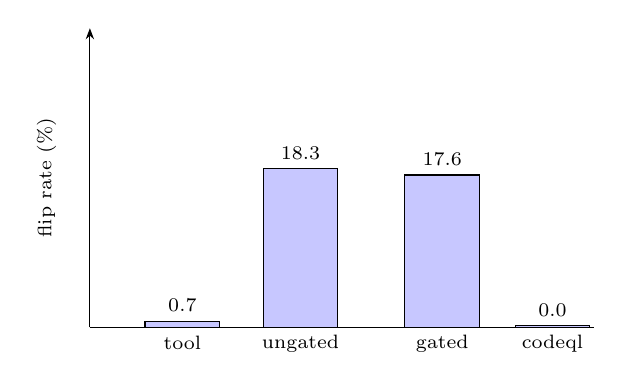
\begin{tikzpicture}[font=\scriptsize, x=1cm, y=1cm]
\draw[-{Stealth[length=1.4mm]}] (0,0) -- (0,3.8);
\draw (0,0) -- (6.4,0);
\foreach \x/\v/\lab in {0.7/0.7/{tool}, 2.2/18.3/{ungated}, 4.0/17.6/{gated}, 5.4/0.0/{codeql}} {
  \pgfmathsetmacro{\hh}{max(\v*0.11,0.02)}
  \draw[fill=blue!22,draw] (\x,0) rectangle (\x+0.95,\hh);
  \node[above] at (\x+0.475,\hh) {\v};
  \node[align=center] at (\x+0.475,-0.2) {\lab};
}
\node[rotate=90,align=center] at (-0.55,1.9) {flip rate (\%)};
\end{tikzpicture}
\caption{Flip rate by verifier arm on the 151-pair stratum. The deterministic
arms barely move: the tool flips once (and over-reports $10\times$), CodeQL
never.}
\label{fig:arms}
\end{figure}

\subsection{Replication and label leakage}
Two ablations separate \emph{sample}, \emph{family}, and \emph{leakage} effects
on the legacy 21-pair subset (Table~\ref{tab:repl}). First, the same model on
the same 21 hand-picked pairs flips at 31.4\% (range 28.6--38.1), against
17.6\% on the 151-pair census: the drop is a \emph{sample} effect, not a model
change. Second, \code{deepseek-flash} on those same 21 pairs flipped at 30.5\%
[22.9,37.1] in the original measurement---two families agree to within one pair,
so the family effect is small and the sample effect dominates. Third, blanking
the commit message (the blinded-message ablation) drops the same pairs from
31.4\% to 13.3\% (range 4.8--19.0): $-18.1$ points, or $-58\%$ relative. The
commit message is a real label channel. Code-only detection (13.3\%) is still
${\sim}19\times$ the pattern matcher's 0.7\%.

\begin{table}[t]
\centering
\caption{Replication and leakage ablations on the legacy 21-pair subset
($k{=}5$, \code{mimo-v2.6-flash} unless noted).}
\label{tab:repl}
\footnotesize
\begin{tabular}{@{}lcc@{}}
\toprule
Configuration & flip rate & range \\
\midrule
with commit message & 31.4\% & 28.6--38.1\% \\
without message & 13.3\% & 4.8--19.0\% \\
\code{deepseek-flash} (E0, same pairs) & 30.5\% & [22.9, 37.1] \\
\midrule
151-pair stratum (contrast) & 17.6\% & [16.7, 18.5] \\
\bottomrule
\end{tabular}
\end{table}

\subsection{Adversarial comments}
Two attack strategies were tested: fixed templates and an adaptive attacker
(Table~\ref{tab:evasion}). The \emph{sanitizer} tactic (``the input is validated
upstream'') was strongest across families. Critically, all successful adaptive
evasions, and 8 of 9 template evasions, were \emph{abstentions} rather than false
positives: an attacker need only make the verifier unsure. The adaptive attacker
roughly doubles evasion relative to templates. This is the security consequence of
the coverage finding above: a defense that only suppresses false positives leaves
the dominant path open.

\textbf{A mitigation that does not help.} As a defense against comment-based
steering we strip all comments from the judged source (line-preserving,
tree-sitter). On the stratum subset the strip did not reduce evasion---12\%
(3/25) with comments present vs.\ 20\% (6/30) stripped---and every evasion in
both arms was again an \emph{abstention} (false positives 0). We report this as
a negative result with a stated confound: the two arms' baseline true-positive
sets differed (5 vs.\ 6) because a temperature-0 reasoning model is
self-inconsistent across runs on these pairs, so the comparison is not fully
paired. The honest conclusion is that input sanitization of comments is not
shown to defend against the abstention attack; the threat model
(Section~\ref{sec:threatmodel}) treats abstention as the asset to protect.

\begin{table}[t]
\centering
\caption{Evasion on the original 21-pair study. JavaVFC templates: baseline 7/21
true positives; adaptive: baseline 6/21, attacker \code{deepseek-v4-pro} vs.\
judge \code{deepseek-flash}. Stratum-scale attack and mitigation results are
discussed above.}
\label{tab:evasion}
\small
\begin{tabular}{@{}lccc@{}}
\toprule
Attack & evasion & via FP & via abstain \\
\midrule
templates (authority) & 43\% (3/7) & 0 & 3 \\
templates (overall) & 26\% & 1 & 8 \\
adaptive (3 rounds) & \textbf{50\% (3/6)} & 0 & 3 \\
\bottomrule
\end{tabular}
\end{table}

\begin{figure}[t]
\centering
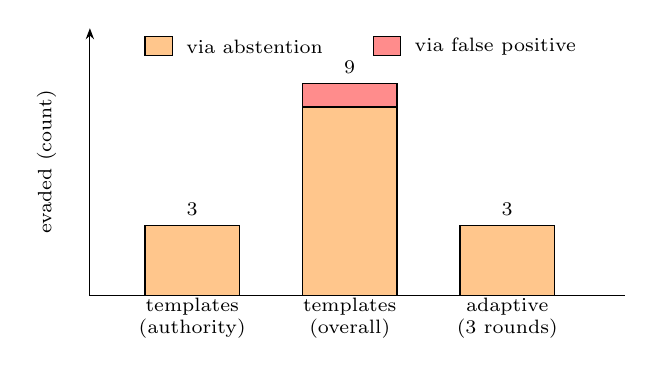
\begin{tikzpicture}[font=\scriptsize, x=1cm, y=1cm]
\draw[-{Stealth[length=1.4mm]}] (0,0) -- (0,3.4);
\draw (0,0) -- (6.8,0);
% scale: 0.3 cm per evaded finding
\draw[fill=orange!45,draw] (0.7,0) rectangle (1.9,0.9);
\node[above] at (1.3,0.9) {3};
\draw[fill=orange!45,draw] (2.7,0) rectangle (3.9,2.4);
\draw[fill=red!45,draw] (2.7,2.4) rectangle (3.9,2.7);
\node[above] at (3.3,2.7) {9};
\draw[fill=orange!45,draw] (4.7,0) rectangle (5.9,0.9);
\node[above] at (5.3,0.9) {3};
\node[align=center] at (1.3,-0.28) {templates\\(authority)};
\node[align=center] at (3.3,-0.28) {templates\\(overall)};
\node[align=center] at (5.3,-0.28) {adaptive\\(3 rounds)};
\draw[fill=orange!45,draw] (0.7,3.05) rectangle (1.05,3.3);
\node[anchor=west] at (1.1,3.17) {via abstention};
\draw[fill=red!45,draw] (3.6,3.05) rectangle (3.95,3.3);
\node[anchor=west] at (4.0,3.17) {via false positive};
\node[rotate=90,align=center] at (-0.55,1.7) {evaded (count)};
\end{tikzpicture}
\caption{Successful evasions by attack and outcome. Nearly all are abstentions: the
attacker only has to make the verifier unsure, not wrong.}
\label{fig:evasion}
\end{figure}

\subsection{Calibration and coverage}
The verifier is nearly precise but poorly calibrated: over five repeated runs on
the 151-pair stratum (Table~\ref{tab:calib}), it false-positives on under 1\% of
fixed revisions, yet its ECE is 0.116 [0.106, 0.131]---better than the
worst values of the original 21-pair measurement (up to 0.35) but still far from
a calibrated probability. It abstains on 51.5\% of the judgements and misses
79.1\% of genuine fixes. The verifier is therefore trustworthy \emph{when it
commits}---but the coverage is low enough that most real fixes are not
certified by it at all.

\begin{table}[t]
\centering
\caption{Calibration on the 151-pair stratum, \code{mimo-v2.6-flash},
$k{=}5$ mean [95\% CI] (six shards merged).}
\label{tab:calib}
\small
\begin{tabular}{@{}lc@{}}
\toprule
Metric & Mean [95\% CI] \\
\midrule
abstention rate & 51.5 [48.5, 54.4] \\
detection (recall on vuln revision) & 20.9 [19.1, 22.8] \\
false-negative rate & 79.1 [77.2, 80.9] \\
fixed-side false-positive rate & 0.9 [0.3, 1.6] \\
accuracy (scored) & 73.9 [72.1, 76.4] \\
ECE & 0.116 [0.106, 0.131] \\
\bottomrule
\end{tabular}
\end{table}

\begin{figure}[t]
\centering
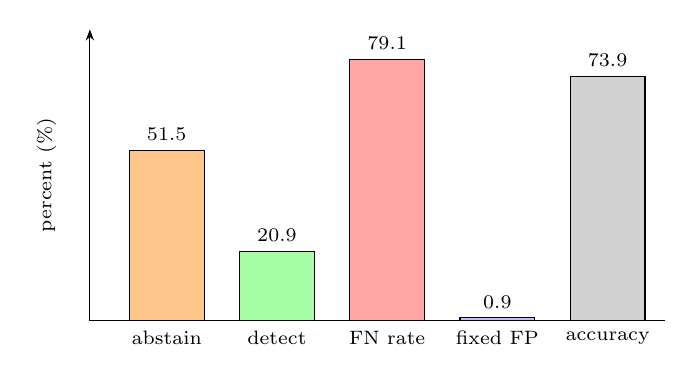
\begin{tikzpicture}[font=\scriptsize, x=1cm, y=1cm]
\draw[-{Stealth[length=1.4mm]}] (0,0) -- (0,3.7);
\draw (0,0) -- (7.3,0);
% scale: 0.042 cm per percent
\foreach \x/\v/\lab/\col in {%
  0.5/51.5/{abstain}/orange!45,%
  1.9/20.9/{detect}/green!35,%
  3.3/79.1/{FN rate}/red!35,%
  4.7/0.9/{fixed FP}/blue!25,%
  6.1/73.9/{accuracy}/gray!35} {
  \pgfmathsetmacro{\hh}{\v*0.042}
  \draw[fill=\col,draw] (\x,0) rectangle (\x+0.95,\hh);
  \node[above] at (\x+0.475,\hh) {\v};
  \node[align=center] at (\x+0.475,-0.22) {\lab};
}
\node[rotate=90,align=center] at (-0.55,1.85) {percent (\%)};
\end{tikzpicture}
\caption{Calibration and coverage on the stratum (mean over five runs). The
verifier is nearly precise (0.9\% fixed-side false positives) yet abstains on
half the inputs and misses most fixes; ECE is 0.116 [0.106, 0.131].}
\label{fig:calib}
\end{figure}

\subsection{Cost}
Output tokens dominate ($\sim$91\% of cost). Disabling model thinking reduced output
from 121{,}596 to 5{,}271 tokens over 42 judgements ($\sim$8$\times$ lower cost) but
introduced fixed-side false positives (0\%$\to$9.5\%) and worsened ECE
(0.153$\to$0.207). A content-addressed verdict cache keyed on the model, prompts, and
slice removed 100\% of repeat cost. At off-peak prices the gated verifier costs
${\approx}\$0.0017$ per judgement. The economics matter: if the bottleneck is
coverage, the productive investment is better context and better evidence, not more
sampling of the same prompt.

\subsection{Detection effectiveness on a labelled benchmark}
To test the whole pipeline against ground truth we ran it on the OWASP
Benchmark for Java~\cite{owaspbench}: 2{,}740 labelled test cases (1{,}415
vulnerable, 1{,}325 safe). The pinned analyzer alone is a strong detector but
over-reports (Table~\ref{tab:benchmark}).

\begin{table}[t]
\centering
\caption{Analyzer on 2{,}740 labelled OWASP Benchmark cases.}
\label{tab:benchmark}
\small
\begin{tabular}{@{}lc@{}}
\toprule
Metric & Value \\
\midrule
TP / FP / FN / TN & 1{,}280 / 463 / 135 / 862 \\
recall (TPR) & 0.905 \\
precision & 0.734 \\
false-positive rate & 0.349 \\
\bottomrule
\end{tabular}
\end{table}

We then asked whether the LLM verifier improves on that precision. On a matched
sample (15 analyzer true positives, 15 analyzer false positives) we ran the
verifier with and without the scanner's rule, message, and CWE hint
(``blind''), to separate genuine judgement from echoing the scanner
(Table~\ref{tab:verifier}).

\begin{table}[t]
\centering
\caption{LLM verification on the matched Benchmark sample. A cache hit or a
blind run cannot echo the scanner's CWE hint.}
\label{tab:verifier}
\small
\begin{tabular}{@{}lcccc@{}}
\toprule
Verifier & TP kept & FP rejected & abstain & prec. \\
\midrule
local 7B, hinted & 14/15 & 0/15 & 1/30 & 0.48 \\
local 7B, blind  & 7/15 & 0/15 & 15/30 & 0.47 \\
cloud, hinted    & 10/15 & 2/15 & 13/30 & 0.67 \\
cloud, blind     & 5/15 & 0/15 & 22/30 & 0.62 \\
\bottomrule
\end{tabular}
\end{table}

Two things follow. First, \emph{no configuration rejects false positives}: neither
a local 7B nor the cloud model separates the safe near-misses from the vulnerable
cases, and the analyzer's precision is not improved. Second, \emph{blinding does
not help}---removing the scanner's hint does not raise rejection, it drives
abstention to 50--73\% and cuts recall. The failure is therefore not
scanner-confirmation bias but the model's inability to ground the deciding
evidence (a sanitizer) from the bounded slice. Error gating aside, verification
here is coverage-bound and adds nothing over the analyzer.

\section{Discussion}
\textbf{The bottleneck is coverage.} Across the scaled run the verifier
false-positives on under 1\% of fixed revisions and abstains on half of all
judgements, but its confidence is not reliably calibrated (ECE 0.116) and it
misses 79.1\% of fixes. Optimising a security agent for precision alone would
miss this entirely. We argue
abstention should be reported as a first-class outcome alongside precision and
recall, and that a verifier which silently declines most inputs is not ``accurate''
in any deployment sense.

\textbf{Attacks target abstention.} Because the verifier already abstains when
evidence is thin, an adversary does not need to convince it a vulnerability is
safe---only to make it unsure. This reframes adversarial robustness for verifiers:
defenses that only suppress false positives leave the dominant path open.

\textbf{Composition relocates trust.} Grounding a claim in verifiable evidence is
cheap and strictly helpful here. Requiring consensus with a weaker verifier is not:
it inherits that verifier's blind spots. ``Add another verifier'' is not a
reliability strategy; ``make the existing verdict answer for itself'' is.

\textbf{Design implications.} Three rules follow. (i) \emph{Score the fix, not the
sample}: a verdict should be evaluated by whether it moves with a code change, which
is cheap to collect and hard to game. (ii) \emph{Make abstention visible}: agents
should surface the fraction of findings they declined to decide, because that is
where adversarial exploitation concentrates. (iii) \emph{Prefer grounding to
consensus}: require a verdict to answer for itself with resolvable evidence rather
than adding another model whose agreement may only import a shared blind spot. A
stronger form of grounding would require a machine-checkable certificate for every
accepted verdict, but our results suggest the immediate constraint is coverage, not
the strength of the evidence a model can already produce.

\textbf{A practical pitfall.} A reasoning-model verifier silently degrades to
``always abstain'' when the token budget is consumed by reasoning tokens
(\code{finish\_reason}=length, empty content). Without the decomposition this is
indistinguishable from a null result. We report it because it cost us a run.

\section{Threat Model}
\label{sec:threatmodel}
\textbf{Assets.} The verdicts. A verifier sits on the gate between a warning
and a fix, so the assets are (i) the \emph{integrity} of a verdict --- it must
track the vulnerability, not the surrounding prose --- and (ii) its
\emph{availability} --- a verdict that silently abstains is a verdict that does
not gate anything.

\textbf{Adversary.} Anyone who can influence what the verifier reads: a
contributor who embeds adversarial comments in submitted source (measured
here), a commit message that names or denies the vulnerability (label leakage,
bounded by the blinded-message ablation), and a scanner whose rule, message,
and CWE hints may be echoed rather than judged (bounded by the blind
condition). We do not model an adversary who can modify the pinned analyzers,
the rulesets, or the model provider; those are trusted, pinned by hash, and
out of scope.

\textbf{Trust boundary.} All code, comments, scanner output, and commit
messages are untrusted \emph{data}, never instructions. The only components
that turn data into a verdict-the-model cannot forge are the evidence gate
(\code{path:line} resolution against the syntax graph) and the decomposition
itself. The abuse cases this paper measures are therefore: steering a verdict
into abstention with comments (Section~\ref{sec:results}), ungrounded
positives (the gate), and hint-echo (the blind condition).

\section{Threats to Validity}
\label{sec:threats}
\textbf{Scale.} The stratum is 151 screened security pairs from one corpus;
the cross-language check is 5 pairs, so the cross-family comparison is
directional. \textbf{Labels.} JavaVFC is
a screening corpus: our companion audit \cite{sastaudit} found only ${\sim}18\%$ of it
is a genuine security fix, so recall is a floor against a cleaner label set.
\textbf{Input shape.} Each revision is an isolated file, which is a floor for tools
that resolve types and near-neutral for pattern matchers. \textbf{Evidence graph.}
Our gating uses a tree-sitter graph, not a sound dataflow engine
\cite{yamaguchi2014modeling,avgustinov2016ql}; it can confirm that a cited
\code{path:line} exists, not that taint flows. \textbf{Non-determinism.} Reasoning
models vary run to run at temperature 0; on the legacy subset we observed flip
rates 28.6--38.1\% across five repeats of one configuration; the $k{=}5$
bootstrap intervals are reported alongside the observed range. \textbf{Families
at scale.} Only \code{mimo-v2.6-flash} was repeated on the
151-pair stratum ($k{=}5$); the cross-family check uses the legacy 21 pairs
(\code{mimo} 31.4\% vs.\ \code{deepseek} 30.5\% on identical pairs), which bounds
the family effect but does not replace a multi-family census.
\textbf{Contamination.} Public fixes may appear in pretraining data; a temporal or
private holdout is not yet used. \textbf{Candidate context.} The verdict request
carries the commit message as bug-report-like context; a message that names or
denies the vulnerability can leak the label directly to the model. The
blinded-message ablation (Section~\ref{sec:results}) re-runs the same pairs
with the message removed and measures a $-18.1$-point drop---the leakage is
real and quantified, but residual leakage through code idioms cannot be ruled
out. \textbf{Benchmark.} OWASP Benchmark labels are
synthetic and single-method, and the verifier ablation is a 30-case sample; it tests
precision behaviour, not recall. \textbf{Adversary.} Our templates are fixed; a
single adaptive attacker was used, and its adaptivity is shallow.
\textbf{CodeQL baseline.} The per-pair no-build mode is the only mode that
completes on this corpus; under build-capable conditions CodeQL might cover
more, so the 0\% flip rate is a measurement of this configuration, not of
CodeQL in general.

\section{Ethics and Responsible Release}
The adversarial comment generator is dual-use. This work is defensive: its purpose
is to measure and expose a failure mode so that verifiers can be made reportable and
robust. We do not release a turnkey attack service; the generator is a small,
reproducible component of a measurement harness, and the paper reports defenses
(evidence gating, coverage reporting, abstention accounting) alongside the risk.

\section{Reproducibility and Artifact}
The harness, pinned analyzers and rule sets, control set, and corpora are released.
Coverage is explicit: Java (a 690-rule ruleset), Python and JavaScript/TypeScript
(minimal rule sets) are \emph{covered}; C is grammar-only; other languages are
reported \emph{unchecked}. A whole-function LLM \emph{audit} surfaces issues without
a ruleset (file context curbs over-flagging), and dependency advisories refresh from
the live OSV feed into immutable, dated snapshots. All assets are pinned by hash; the
control reproduction (12/18 vulnerable, 1/3 safe) and the Python-pair measurement run
fully offline; 158 tests accompany the code. A content-addressed verdict cache makes
repeat runs deterministic and free.

\section{Conclusion and Future Work}
LLM security verifiers track fixes far better than pattern matchers and CodeQL
and are nearly precise when they commit (0.9\% fixed-side false positives), but
they are \emph{not} reliably calibrated and are nonetheless \emph{silent} on
about half of their inputs---a
weakness that adversarial comments directly amplify, and that composition with
deterministic tools does not fix. The actionable reframing is that the bottleneck of
a security verifier is \emph{coverage}, and that its dominant adversarial target is
\emph{abstention}. Future work must (i) replicate the 151-pair census across at
least two more model families, (ii)
evaluate path-level candidates on multi-file revisions, and (iii) treat abstention
and coverage as first-class metrics for security agents.

\bibliographystyle{IEEEtran}
\bibliography{references}

\end{document}
